\chapter{Introduction and Motivation}
\label{sec:part1-motivation}

% \hl{copied from glenside intro}
% Machine learning (ML) and other
%   high-performance computing (HPC)
%   applications increasingly rely on
%   specialized hardware accelerators to
%   provide speed and energy efficiency~\cite{jouppi2017tpu, krizhevsky2012conv, reuther2019survey}.
% This trend has highlighted the need
%   for flexible accelerator support
%   in domain-specific compilers like
%   Halide~\cite{halide},
%   TVM~\cite{chen2018tvm},
%   TensorFlow/MLIR~\cite{tensorflow, mlir}, and
%   PyTorch~\cite{pytorch}.

% Adding accelerator support to
%   an existing compiler typically
%   uses custom pattern matching to
%   map expensive tensor operations
%   from applications down to
%   accelerator invocations~\cite{
%     yang2020interstellar, byoc}.
% Pattern matching often additionally relies on
%   various other transformations
%   to canonicalize intermediate representations (IRs)
%   %~\cite{??}
%   and massage data layouts into
%   formats matching accelerator requirements~\cite{nvidia2020nhwc}.
% Even with these changes,
%   users may need to manually modify their application to
%   help the compiler discover opportunities
%   for dispatching operations to accelerators, 
%   such as by changing data types or unrolling loops.
% \hl{end copied from glenside intro}

% Top-level points: 
% We need something like the 3LA methodology;
% 3LA methodology needs flexible matching.


% WE NEED SOMETHING LIKE 3LA METHODOLOGY
% Points:
%% Hardware acceleration is important.
%% Accelerators are nothing without testing/without compilers? which one?
%% Need a methodology for building compilers.

%% Hardware acceleration is important.

Hardware acceleration has powered significant advances
  in subfields like artificial intelligence, image processing, and graph analysis~\cite{han2016eie,chen2016eyeriss,reagen2016minerva,zhang2016cambricon,hameed2010understanding,ham2016graphicionado,jouppi2017tpu, krizhevsky2012conv, reuther2019survey}.
This trend has highlighted the need
  for flexible \gls{accelerator} support
  in domain-specific compilers like
  Halide~\cite{halide},
  TVM~\cite{chen2018tvm},
  TensorFlow/MLIR~\cite{abadi2016tensorflow,mlir}, and
  PyTorch~\cite{pytorch}.

Despite our increasing dependence
  on accelerators,
  building compilers
  for custom accelerators
  remains a daunting task.
Developing a compiler
  for a custom accelerator
  requires significant
  \cref{thesis:devtime}.
Current frameworks for compiler generation
  generally require significant compilers expertise,
  and the sheer amount of effort
  required to build a compiler from the ground up
  generally limits bespoke compiler construction
  to teams
  at large companies,
  e.g. the TensorFlow 
  stack~\cite{abadi2016tensorflow}
  for Google's 
  TPU~\cite{jouppi2017tpu,jouppi2020tpu}.
Though projects
  such as 
  MLIR~\cite{mlir,
  lattner2021mlir,
  eldridge2021mlir}
  and
  Exo~\cite{ExoPldi22}
  have begun to prescribe
  a general framework
  for structuring a compiler,
  these tools are built for
  domain experts,
  and require significant time investment.
% There is a need for
%   automated techniques
%   for compiler generation,
%   to lower the barrier
%   and allow non-experts to generate
%   functioning compilers.
% An example of such a technique
%   is the deep learning compiler
%   TVM's~\cite{chen2018tvm}
%   Bring Your Own Codegen (BYOC)
%   framework~\cite{chen2021byoc}.
% However,
%   though BYOC makes it easy for
%   users to add basic support
%   for accelerators,
%   we will see 
%   that its ability to 
%   match workloads to accelerators
%   is lacking---%
%   a hole that automated methods can fill.
Even once a compiler
  is constructed
  for a piece of custom hardware,
  it may still miss crucial
  \cref{thesis:optimizations}---%
  in this case, taking the form of
  accelerator mapping opportunities.
% Enabling a compiler to realize
%   that a certain operator
%   in a workload
%   can be run on an accelerator,
%   for example,
%   may require syntactic changes
%   to the input program,
%   especially when using
%   a matcher like
%   TVM's BYOC.

Furthermore, the difficulty in building compilers
  for accelerators
  has a negative effect
  on accelerator 
  \cref{thesis:correctness}.
Core to ensuring correctness of
  accelerators
  is the process of end-to-end
  hardware \gls{validation}---%
  that is, testing the hardware design
  on full applications---%
  and thorough hardware validation
  requires a working compiler.
Some accelerator bugs 
  will only be caught
  during
  full-application validation,
  especially bugs in the
  microarchitectural optimizations common in accelerator design~\cite{chan2014itrs,fang2019understanding,lai2021programming}.
For example,
  a deep learning
  accelerator may use
  a custom numeric format
  tuned to be storage-efficient,
  while still providing enough
  precision
  to support effective inference.
Testing the numeric format
  on a single layer
  of the deep learning model
  may produce results
  well within the designer's
  error bounds.
However, if the designer
  neglects to test
  \textit{all}
  layers of the model,
  they may fail to discover that,
  even though individual layers
  behave well,
  the error may accumulate
  across layers,
  producing inaccurate application-level results~\cite{zorn2021rounding}.
Early end-to-end application level validation is thus essential
  for avoiding expensive and complex late stage hardware design changes.

\begin{figure}
\centering
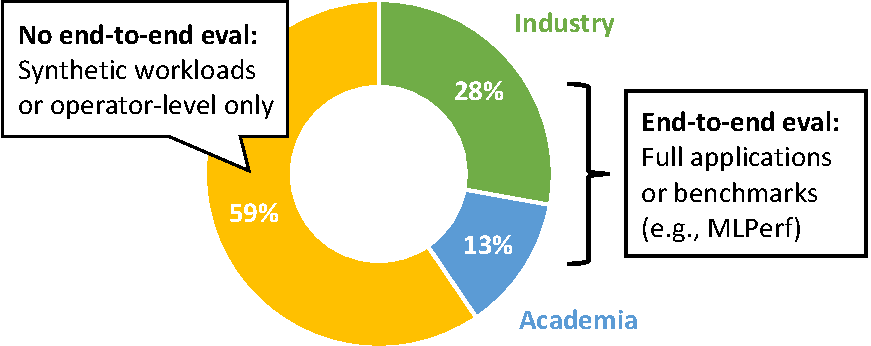
\includegraphics[width=.6\textwidth]{assets/3la-pie.pdf}
\caption{
\textit{This figure is reproduced
  from Huang et al.~\cite{huang2024application}.}
\textbf{Gap in end-to-end evaluation of accelerators for neural network applications:} 
Survey of papers from ISCA, MICRO, VLSI, and ISSCC in 2021 and ICCAD, DAC in 2020.
The authors surveyed $79$ papers introducing new DL accelerator designs/methodologies and determined how each accelerator was evaluated. Only 41\% of the works reported end-to-end evaluation on non-synthetic applications, of which 68\% (28\% of the total) were from industrial teams.
}
\label{fig:3la-pie}
\end{figure}


The difficulty in building compilers
  is reflected in the literature.
\Cref{fig:3la-pie} presents a figure
  originally published in
  Huang et al.~\cite{huang2024application},
  which shows how few
  new accelerator designs
  were evaluated on end-to-end applications.
As we will see,
  this has practical consequences,
  as bugs in these accelerators
  may not be apparent
  until full end-to-end
  validation.

In response to the challenges
  of hardware validation
  to the common designer,
  Huang et al.~(including
    the author of this dissertation)
  developed
  3LA:
  a methodology
  to make testing
  easier for new accelerator designs~\cite{huang2022specialized,huang2024application}.
The \TLA flow
  is shown in 
  \cref{fig:3la-diagram}.
The primary contribution of 3LA
  is 
  a methodology to end-to-end evaluate accelerators on unmodified, full applications.
While 3LA as a whole
  is not a contribution of this dissertation
  (see the dissertations of Bo-Yuan Huang~\cite{huang2022specialized}
    and Steven Lyubomirsky~\cite{lyubomirsky2022compiler}),
  the motivations behind 3LA 
  and the story of its development
  are important for \cref{part:glenside-and-3la}
  of this dissertation.

\begin{figure}
    \centering
    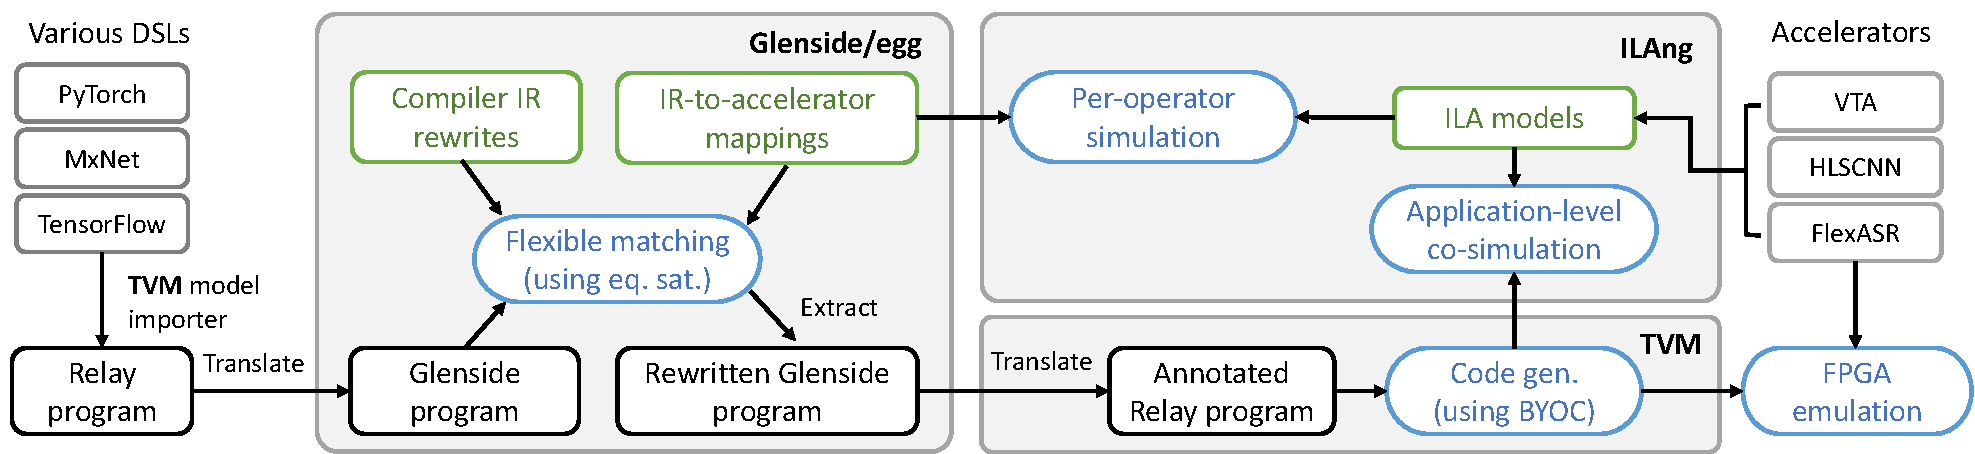
\includegraphics[width=\textwidth]{assets/3la-diagram.pdf}
    \caption{
\textit{This figure is reproduced from
  Huang et al.~\cite{huang2024application}.}
Diagram of the 3LA prototype's flow.
Note that only the ``Glenside/egg''
  portion of 3LA
  is considered a contribution
  of this dissertation;
  for more information on the other components,
  please see the original paper.
}
    \label{fig:3la-diagram}
\end{figure}

3LA solves two major problems,
  the first being that
  generating simulators
  for hardware
  is difficult
  and time consuming.
% Second, even given a simulator
%   for your design,
%   it is then difficult
%   to run full applications
%   on the simulator.
3LA solves this problem
  using the Instruction-Level Abstraction (ILA)~\cite{huang2018instruction,huang2018formal}.
ILA is a specification system
  originally designed for
  system-on-chip verification purposes.
The authors of 3LA
  repurposed the ILA
  as a tool for capturing
  and simulating
  machine learning accelerator behavior,
  giving accelerator developers
  a framework for generating fast,
  high-level simulators
  for their accelerators.
The first contribution
  of 3LA
  we do not consider
  a contribution of this dissertation;
  again, please refer to the dissertations
  of the coauthors
  for more information about 3LA as a whole.

The second challenge 3LA solves
  is that,
  even given a simulator,
  compiling
  full programs to the simulator
  is difficult.
At the time of developing 3LA,
  there were few open-source, flexible 
  compiler frameworks
  for targeting custom hardware.
One open-source framework
  supporting mapping
  to custom accelerators
  is TVM's Bring Your Own Codegen (BYOC)~\cite{byoc,chen2021byoc}.
Initially, the 3LA authors
  attempted to use BYOC
  to address their second issue.
To use BYOC, the user
  provides syntactic patterns
  which BYOC then searches for
  in the workloads of interest.
However,
  exact syntactic pattern matching 
  (which we refer to simply as
    ``exact matching'')
  faces difficulties
  as there is often no canonical way
  to represent an operation,
  necessitating either the addition of more patterns
  or manual modifications to the input program
  to match the expected patterns.
Application code can vary greatly in structure,
  particularly in the case of compiler IRs,
  which may be produced after several iterations
  of program transformations.
Code variations are especially prevalent
  in machine learning compilers,
  where workloads are often imported
  from other languages via importers.
Even for the same machine learning model,
  importers from different languages
  can produce wildly different (but equivalent)
  imported programs.
Consider, for example,
  the compiler IR pattern for a linear layer
  in 
  LSTM-WLM:
\small
\[ \texttt{(bias\_add (nn\_dense \%a \%b) \%c)}. \]
\normalsize
However, 
  in another model (ResNet-20)
  the linear layers are equivalently expressed as: 
\small
\[ \texttt{(add (reshape (nn\_dense \%a \%b) \%s) \%c)} \]
\normalsize
when \instrInText{\%c} is a vector, for certain shapes \instrInText{\%s}.
%
Though they are \textit{semantically}
  equivalent,
  they are not \textit{syntactically}
  equivalent,
  and thus
  we cannot match both of these operations
  with
  a single syntactic pattern.
With an inflexible system like BYOC,
  we would be forced to add
  a new pattern for each possible
  way of writing
  the operator of interest.
To put this in the framing of my dissertation,
  BYOC is near the bottom-left corner
  on our model explicitness--algorithm adaptability spectrum
  in \cref{fig:intro:model-alg-spectrum}.
BYOC's \cref{thesis:models}
  of hardware are explicit:
  rewrites, capturing the functioning of hardware.
However, its \cref{thesis:algorithms}---%
  the underlying exact matching algorithm---%
  is inflexible,
  unable to find semantically equivalent
  but syntactically different
  matches.


This is where I was able to apply
  my dissertation.
When existing \cref{thesis:algorithms}
  (exact matching)
  proved inflexible,
  we introduced a new algorithm
  (\gls{equality-saturation})
  whose increased flexibility
  made it easier to find opportunities
  to invoke accelerators.
We developed a language
  called \g
  which allowed for the application
  of equality saturation
  to the task of accelerator mapping.
We then integrated \g in 3LA
  to solve the second challenge listed above.

Note that we do not improve upon
  model explicitness
  in \cref{part:glenside-and-3la};
  notice that the point for \g
  is above, but not further to the right of,
  the point for BYOC
  on \cref{fig:intro:model-alg-spectrum}.
Both \g and BYOC use similar patterns
  to capture the functioning of hardware.
In \cref{part:lakeroad},
  we will show how we can increase
  both algorithm adaptability
  \textit{and}
  model explicitness.


The rest of \cref{part:glenside-and-3la}
  proceeds as follows.
In \cref{chapter:part1-glenside},
  we introduce \g.
In \cref{chapter:part1-evaluation},
  we evaluate \g,
  primarily by demonstrating what
  \g is able to achieve
  when integrated into 3LA.
In \cref{chapter:part1-background},
  we present related work.


% 3LA methodology needs flexible matching.
% \section{Summary of the 3LA Methodology}

% \hl{probably delete}

% The 3LA methodology as a whole
%   (or just 3LA for short)
%   is not a contribution of this dissertation---%
%   see the dissertations of
%   Bo-Yuan Huang~\cite{huang2022instruction}
%   and 
%   Steven Lyubomirsky%
%   ~\cite{lyubomirsky2022compiler}.
% However,
%   \g, a contribution of this dissertation,
%   is a 
%   significant component of 3LA,
%   and its development 
%   is inextricably linked to the development
%   of 3LA.
% As such,
%   some understanding of the 3LA
%   methodology
%   is required for understanding
%   \g.
  


% \hl{
% Copied from 3LA paper, rephrase: 
% }

% The ILA is an ISA-like formal model 
%   for specifying the functional behavior of accelerators.
% It generalizes the ISA to accelerators, 
% %and provides a modular functional specification as a set of instructions. Each 
%   where each 
%   instruction of an accelerator ILA corresponds 
%   to a command at the accelerator interface, i.e., an MMIO load or store from a host processor.
% Like processor ISAs, 
%   the ILA captures a formal semantics of the accelerator behavior, by specifying how each instruction 
%   reads or updates software-visible (viz., architectural) state variables in the accelerator,
%   while abstracting out implementation details. 
  
% Fig.~\ref{fig.ila-example} shows an example
%   ILA specification for one of the instructions of FlexASR~\cite{tambe20219} (one of the three accelerators used in our evaluation studies). The ILA models are written in ILAng, a DSL embedded in C++. The figure caption points out the per-instruction modular specification, where each instruction is specified by defining its decode condition (i.e., when the instruction is triggered) and state update functions (i.e., how it updates
%   the architectural state variables). 
%   %updates are specified.

% Thus far, the ILA has been used only for accelerator implementation verification and co-verification of firmware~\cite{huang2018formal,huang2018instruction}.
% In this work, we use ILA as a formal SW/HW interface that drives the key tasks in compilation and application-level testing for accelerators.

% \hl{end copy from 3LA }